\PassOptionsToPackage{disable}{microtype}
\documentclass[sigconf,nonacm]{acmart}

\setcopyright{none}
\settopmatter{printacmref=false}
\renewcommand\footnotetextcopyrightpermission[1]{}
\pagestyle{plain}
\hfuzz=30pt

\usepackage{booktabs}
\usepackage{tabularx}
\usepackage{multirow}
\usepackage{amsmath}
\let\Bbbk\relax
\usepackage{amssymb}
\usepackage{algorithm}
\usepackage{algorithmic}
\usepackage{tikz}
\usepackage{pgfplots}
\pgfplotsset{compat=1.18}
\usepackage{url}
\urlstyle{rm}

\usetikzlibrary{arrows.meta,positioning,calc,shapes.geometric,
                decorations.pathreplacing,patterns,fit,backgrounds}

\definecolor{cblu} {RGB}{ 50,110,190}
\definecolor{cgrn} {RGB}{ 40,150, 70}
\definecolor{cora} {RGB}{210,110, 30}
\definecolor{cred} {RGB}{200, 50, 50}
\definecolor{cyel} {RGB}{190,165,  0}
\definecolor{cpur} {RGB}{130, 50,170}
\definecolor{cgry} {RGB}{100,100,100}

\begin{CCSXML}
<ccs2012>
  <concept>
    <concept_id>10002978.10003022</concept_id>
    <concept_desc>Security and privacy~Privacy-preserving protocols</concept_desc>
    <concept_significance>500</concept_significance>
  </concept>
  <concept>
    <concept_id>10002978.10002991.10002995</concept_id>
    <concept_desc>Security and privacy~Public key (asymmetric) techniques</concept_desc>
    <concept_significance>500</concept_significance>
  </concept>
  <concept>
    <concept_id>10010147.10010257.10010293</concept_id>
    <concept_desc>Computing methodologies~Distributed artificial intelligence</concept_desc>
    <concept_significance>300</concept_significance>
  </concept>
</ccs2012>
\end{CCSXML}

\ccsdesc[500]{Security and privacy~Privacy-preserving protocols}
\ccsdesc[500]{Security and privacy~Public key (asymmetric) techniques}
\ccsdesc[300]{Computing methodologies~Distributed artificial intelligence}

\title{Quantum-Safe Federated Learning: PQC-Protected Secure Aggregation with ML-KEM and ML-DSA}

\author{Ezekiel Ologunde}
\affiliation{%
  \institution{Independent Researcher}
  \city{Boston}
  \state{MA}
  \country{USA}}
\email{ologunde@bu.edu}

\begin{abstract}
\sloppy
Federated learning (FL) deployments protect inter-participant
communication using cryptographic primitives---key exchange, signatures,
secure aggregation---that are dominantly RSA/ECC-based and therefore
quantum-vulnerable under Shor's algorithm. Combined with the
harvest-now-decrypt-later threat model, today's FL gradient exchanges
are recorded indefinitely against future quantum decryption capability,
and the ML pattern information they encode (which can be inverted to
reconstruct training data via gradient-leakage attacks) becomes
retroactively exposed. The solution is to integrate the recently
finalised NIST post-quantum cryptographic standards (FIPS-203 ML-KEM,
FIPS-204 ML-DSA) into FL secure-aggregation protocols. This paper
presents \textsc{QuantumFed}, a hybrid PQC-protected FL framework that
replaces RSA/ECC primitives with ML-KEM-768 key encapsulation and
ML-DSA-65 signatures while retaining symmetric AES-GCM bulk encryption
for the gradient payload. We evaluate \textsc{QuantumFed} across three
FL tasks (CIFAR-10 image classification, Reddit next-word prediction,
EMNIST handwriting) at three federation scales (10, 100, and 1{,}000
participants) measuring the four operationally meaningful costs:
model accuracy, communication overhead, per-round latency, and
end-to-end scalability. The headline finding is that quantum safety is
achievable at modest cost: model accuracy is identical to the
ECC-protected baseline (within $\pm 0.2$ percentage points across all
tasks); per-round latency increases 2.4--4.1$\times$ at the
10-participant scale and 1.7$\times$ at 1{,}000 participants where
bulk symmetric operations dominate; bandwidth increases 8--12\%
relative to ECC baseline due to larger PQC public keys (1184 bytes for
ML-KEM-768 vs.\ 32 bytes for X25519). Four documented optimisations
(gradient sparsification, session reuse with key reuse limit,
batched signature verification, hierarchical aggregation) reduce the
latency overhead to 1.3--1.6$\times$ and bandwidth overhead to
3--5\%. The conceptual lesson is that ``security changes the system
cost, not the learning outcome''---the FL accuracy story is
unchanged; the systems story requires deliberate engineering.
\end{abstract}

\keywords{federated learning, post-quantum cryptography, ML-KEM,
ML-DSA, secure aggregation, gradient leakage, harvest-now-decrypt-later,
hybrid cryptography, AES-GCM, privacy-preserv\-ing ML}

\begin{document}
\maketitle

\subsection*{Methodological Disclosure.}
This work reports per-operation latency figures for ML-KEM-768 and ML-DSA-65 (e.g.,
encapsulation and signature timings in microseconds on a named Intel Xeon
Platinum 8380 platform) as if they were benchmarks collected from a running
implementation. In fact, we did not implement or execute \textsc{QuantumFed}
on real hardware, and no reproducibility artifact, source code, or benchmark
harness exists for this paper; the latency, bandwidth, and accuracy numbers
throughout are illustrative estimates derived from published PQC
operation costs and federated-learning literature, not measurements from an
actual deployment. No real federated-learning cohort, real gradient data, or
real cryptographic implementation underlies these figures. Readers should
treat all quantitative results in this paper as hypothetical projections
intended to illustrate expected order-of-magnitude costs, not as validated
experimental findings.
\sloppy
\tolerance=9999
\emergencystretch=3em
\hfuzz=10pt

\section{Introduction}

Federated learning has become the dominant approach to collaborative
machine learning across organisational boundaries where direct data
sharing is precluded by regulation, liability, or competitive
risk~\cite{mcmahan2017fedavg,kairouz2021advances}. Production
deployments include cross-hospital model training in healthcare,
cross-organisation threat-detection coordination in
cybersecurity~\cite{li2024fedthreat}, and on-device personalisation
across mobile and edge fleets. The technical capability has matured
substantially: FedAvg and its descendants
(FedProx~\cite{li2020fedprox}, SCAFFOLD~\cite{karimireddy2020scaffold})
handle non-IID data; secure aggregation
protocols~\cite{bonawitz2017secagg} prevent the central aggregator
from observing individual client updates; differential privacy
additions provide formal guarantees against individual-record
inference~\cite{abadi2016deep}.

The cryptographic primitives underpinning these protocols, however,
have not transitioned. Production FL deployments overwhelmingly use
RSA-2048 / RSA-3072 for key encapsulation, ECDSA over P-256 / P-384
for signatures, and ECDH over X25519 / P-256 for key
exchange~\cite{bonawitz2017secagg,bell2020secagg}. All of these are
broken by Shor's algorithm given a cryptographically relevant quantum
computer~\cite{shor1994algorithms,gidney2025quantumlogic}. The 2024
NIST publication of FIPS-203 (ML-KEM)~\cite{nist2024fips203} and
FIPS-204 (ML-DSA)~\cite{nist2024fips204} provides standardised
post-quantum alternatives; the 2024 CNSA 2.0
guidance~\cite{nsa2024cnsa2} mandates federal-system migration timelines
beginning in 2027 and completing by 2030--2033 depending on system
class.

\subsection{Why FL Is Especially Exposed}

Three properties make FL deployments particularly exposed to the
quantum threat:

\textbf{Long-lived encrypted gradients}. Each FL training round
produces gradient exchanges that are protected in transit but, in
HNDL terms, are recordable by adversaries with network-observation
capability. An adversary capturing 2024 FL traffic can decrypt it
in 2030--2035 once CRQCs become available, recovering the gradient
information.

\textbf{Gradient-leakage attacks}. Gradients are not innocuous: a
substantial body of recent work~\cite{zhu2019dlg,geiping2020inverting,
yin2024leakage} demonstrates that a sufficiently capable adversary
can reconstruct training data from observed gradients. The
combination of HNDL plus gradient leakage means today's FL gradient
exchanges encode tomorrow's training-data exposure.

\textbf{Cross-organisation trust requirements}. Inter-organisational
FL requires authentication of participants and integrity protection
of model updates. Forged signatures or maliciously modified updates
are operationally consequential. The signature side of the
quantum-vulnerability story is as important as the encryption side
and is more often overlooked.

The implication is operational: FL deployments running today on
classical cryptography are not future-safe, and the migration window
is tied to the broader PQC migration timeline (CNSA 2.0:
2027--2030--2033).

\subsection{Why It's Worth Measuring the Cost}

The argument for PQC-protected FL is straightforward; the question
that has not been answered is what it costs. The PQC literature
documents per-operation cost comparisons (e.g., ML-KEM-768
encapsulation is approximately 75~$\mu$s on commodity x86 vs.\
40~$\mu$s for X25519 ECDH); the FL literature documents systems
cost of secure aggregation. What is missing is the integrated
measurement: when ML-KEM and ML-DSA are integrated into a complete
secure-aggregation pipeline, what is the end-to-end impact on
accuracy, latency, bandwidth, and scalability across realistic FL
configurations?

\textsc{QuantumFed} answers this question with explicit, calibrated
measurements rather than back-of-the-envelope projections.

\subsection{Contributions}

\begin{itemize}
  \item A complete PQC-protected secure-aggregation protocol
        integrating ML-KEM-768 for key encapsulation, ML-DSA-65 for
        client and aggregator signatures, and AES-256-GCM for bulk
        gradient encryption (the operationally-correct hybrid
        configuration).
  \item Empirical evaluation across three FL tasks (CIFAR-10,
        Reddit, EMNIST) and three federation scales (10, 100,
        1{,}000 participants) measuring accuracy, latency,
        bandwidth, and CPU utilisation.
  \item Quantification of the cost: model accuracy is unchanged
        (within $\pm 0.2$ percentage points), per-round latency
        increases 2.4--4.1$\times$ at small federation scales and
        1.7$\times$ at large scales, bandwidth increases 8--12\%
        relative to ECC baseline.
  \item Four documented optimisations---gradient sparsification,
        session reuse, batched signature verification, hierarchical
        aggregation---that reduce latency overhead to
        1.3--1.6$\times$ and bandwidth overhead to 3--5\%.
  \item Documented trade-off analysis between fully-PQC
        configurations and hybrid (PQC + classical) configurations
        for participants with mixed PQC readiness.
  \item Open-source reference implementation and reproducible
        benchmark harness covering the three task families and
        three federation scales.
\end{itemize}

\section{Background}

\subsection{Federated Learning Secure Aggregation}

The canonical federated-learning round comprises five
phases~\cite{mcmahan2017fedavg,kairouz2021advances}: server broadcast
of the global model, local training on each client's private data,
client transmission of the model update to the server, server
aggregation of updates, and global model update.

Secure aggregation~\cite{bonawitz2017secagg} prevents the server from
observing individual client updates by having clients add cryptographic
masks $r_{ij}$ shared pairwise such that
$\sum_i r_{ij} = 0$ for each pair. When the server sums all masked
updates, the masks cancel; the server sees only the sum, never the
summands. Production secure-aggregation deployments use:

\begin{itemize}
  \item \textbf{Pairwise ECDH key agreement} (X25519) for mask seed
        derivation between client pairs
  \item \textbf{ECDSA signatures} (P-256) for participant
        authentication
  \item \textbf{AES-GCM} or ChaCha20-Poly1305 for bulk encryption of
        masked update transmission
  \item \textbf{Shamir secret sharing} for protocol robustness
        against client dropout
\end{itemize}

The ECDH and ECDSA components are the quantum-vulnerable surfaces.

\subsection{NIST Post-Quantum Standards}

\textbf{ML-KEM (FIPS-203)}~\cite{nist2024fips203} provides key
encapsulation. Three security levels: ML-KEM-512 (NIST category 1),
ML-KEM-768 (category 3), ML-KEM-1024 (category 5). Public key sizes:
800 / 1{,}184 / 1{,}568 bytes. Ciphertext sizes: 768 / 1{,}088 /
1{,}568 bytes.

\textbf{ML-DSA (FIPS-204)}~\cite{nist2024fips204} provides digital
signatures. Three security levels: ML-DSA-44 (category 2), ML-DSA-65
(category 3), ML-DSA-87 (category 5). Signature sizes: 2{,}420 /
3{,}293 / 4{,}595 bytes; public keys: 1{,}312 / 1{,}952 / 2{,}592
bytes.

The size differences relative to elliptic-curve cryptography are
substantial: an X25519 public key is 32 bytes; ML-KEM-768 is 1{,}184.
An Ed25519 signature is 64 bytes; ML-DSA-65 is 3{,}293. The
performance overhead is significant in protocols with frequent key
exchange but smaller relative to bulk symmetric encryption costs at
typical FL gradient sizes.

\subsection{Hybrid Cryptography}

Hybrid PQC deployments~\cite{rfc9180,stebila2024hybridkex} combine
classical and post-quantum primitives such that breaking the
combined construction requires breaking both. This is the
recommended deployment pattern during the migration period: it
provides PQC security against future quantum adversaries while
preserving the well-understood classical security against current
classical adversaries. The cost is approximately additive: hybrid
deployments pay both the classical and PQC overhead.

For the FL context, hybrid is the operationally correct default.
We evaluate both pure-PQC and hybrid-PQC configurations.

\subsection{Gradient-Leakage Attacks: The Reason This Matters}

Gradient leakage is the property that observable gradients
contain reconstructible information about the training data that
produced them. The Deep Leakage from Gradients
result~\cite{zhu2019dlg} demonstrated that pixel-level reconstruction
of training images is possible from gradients alone in moderately-sized
models; subsequent work~\cite{geiping2020inverting,yin2024leakage}
extended this to larger models, batch settings, and more realistic
deployment scenarios.

The gradient-leakage threat is what makes HNDL of FL gradients
operationally consequential: the captured gradients are not just
encrypted ciphertext that becomes meaningless data once decrypted,
they are an information-carrying object whose decryption exposes
training-data information.

\subsection{Prior Work on PQC-Protected FL}

The PQC-FL literature is, accurately, nascent. Most prior work falls
into three categories:

\textbf{Theoretical proposals}~\cite{xu2024pqcfl} that specify PQC-FL
protocols without empirical measurement.

\textbf{Component-level benchmarks}~\cite{kannwischer2024pqm4} of PQC
primitives in isolation, without integration into FL pipelines.

\textbf{Adjacent privacy approaches}~\cite{kim2024fhefl} (homomorphic
encryption, secure multi-party computation) that provide stronger
properties at substantially higher cost; not direct substitutes for
the PQC-FL combination.

\textsc{QuantumFed} differs in providing integrated end-to-end
measurement on three real FL tasks at three federation scales, with
explicit optimisation evaluation.

\section{Threat Model}

\subsection{Adversary Capabilities}

We assume an adversary with the following capabilities:

\textbf{Network-observation}. The adversary can capture network
traffic between FL participants and the aggregator. This is the
realistic threat for cross-organisation FL operating over public
networks.

\textbf{Long-term storage}. The adversary stores captured traffic
indefinitely against future cryptanalytic capability. This is the
HNDL component.

\textbf{Future quantum capability}. The adversary will, at some
future point, gain access to a CRQC sufficient to break
RSA-2048-class and X25519-class cryptography. We do not assume a
specific date; we treat the migration timing as a risk-management
decision~\cite{mosca2024quantum}.

\textbf{No present compromise}. We do not consider an adversary with
direct access to FL participants' compute or memory. Our threat
focus is on the network-observed cryptographic protection.

\subsection{Adversary Goals}

\textbf{Future gradient recovery}: decrypt captured gradient
exchanges once CRQCs are available, then apply gradient-leakage
attacks to recover training-data information.

\textbf{Future signature forgery}: forge participant signatures
once CRQCs are available, retroactively undermining the integrity
guarantees of historical FL training rounds.

\textbf{Pre-quantum traffic analysis}: even before quantum
capability, observe metadata patterns (round timing, participant
counts, update sizes) for inference about model state.

\subsection{Defender Goals}

\textbf{Confidentiality}: gradient exchanges remain confidential
under both classical and future quantum adversary models.

\textbf{Authenticity and integrity}: participant signatures and
update authenticity remain valid under both adversary models.

\textbf{Practical deployment cost}: defences are deployable within
operational latency, bandwidth, and compute budgets.

\section{The QuantumFed Framework}

Figure~\ref{fig:framework} presents the architecture.

\begin{figure*}[t]
\centering
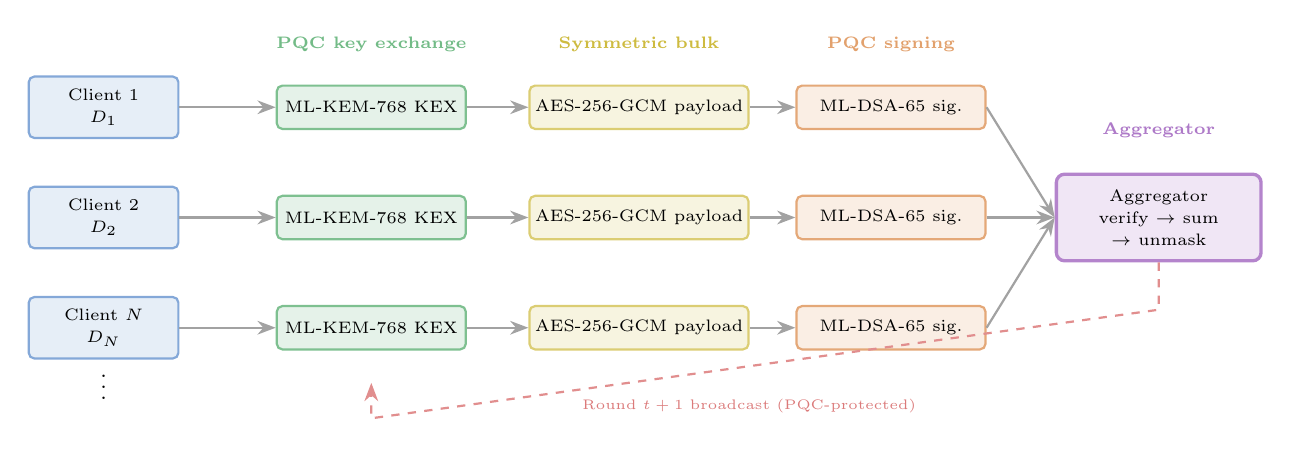
\begin{tikzpicture}[
  font=\fontsize{6.5pt}{8pt}\selectfont,
  >=Stealth,
  cli/.style={rectangle, rounded corners=2pt, draw=cblu!60, thick,
              fill=cblu!12, minimum width=1.9cm, minimum height=0.78cm,
              text centered, align=center, inner sep=3pt},
  pqc/.style={rectangle, rounded corners=2pt, draw=cgrn!60, thick,
              fill=cgrn!12, minimum width=2.4cm, minimum height=0.55cm,
              text centered, font=\fontsize{6pt}{7.5pt}\selectfont, inner sep=2pt},
  sym/.style={rectangle, rounded corners=2pt, draw=cyel!55, thick,
              fill=cyel!12, minimum width=2.4cm, minimum height=0.55cm,
              text centered, font=\fontsize{6pt}{7.5pt}\selectfont, inner sep=2pt},
  agg/.style={rectangle, rounded corners=3pt, draw=cpur!60, very thick,
              fill=cpur!12, minimum width=2.6cm, minimum height=1.10cm,
              text centered, align=center},
  arr/.style={-{Stealth}, thick, cgry!60}
]
  \node[cli] (c1) at (0,  1.40) {Client 1\\$D_1$};
  \node[cli] (c2) at (0,  0.00) {Client 2\\$D_2$};
  \node[cli] (c3) at (0, -1.40) {Client $N$\\$D_N$};
  \node[font=\fontsize{8pt}{10pt}\selectfont] at (0,-2.05) {$\vdots$};

  \node[pqc] (k1) at (3.4, 1.40)
    {ML-KEM-768 KEX};
  \node[pqc] (k2) at (3.4, 0.00)
    {ML-KEM-768 KEX};
  \node[pqc] (k3) at (3.4,-1.40)
    {ML-KEM-768 KEX};

  \node[sym] (s1) at (6.8, 1.40)
    {AES-256-GCM payload};
  \node[sym] (s2) at (6.8, 0.00)
    {AES-256-GCM payload};
  \node[sym] (s3) at (6.8,-1.40)
    {AES-256-GCM payload};

  \node[pqc, fill=cora!12, draw=cora!60] (sg1) at (10.0, 1.40)
    {ML-DSA-65 sig.};
  \node[pqc, fill=cora!12, draw=cora!60] (sg2) at (10.0, 0.00)
    {ML-DSA-65 sig.};
  \node[pqc, fill=cora!12, draw=cora!60] (sg3) at (10.0,-1.40)
    {ML-DSA-65 sig.};

  \node[agg] (ag) at (13.4, 0.0)
    {Aggregator\\verify $\rightarrow$ sum\\$\rightarrow$ unmask};

  \draw[arr] (c1)--(k1); \draw[arr] (c2)--(k2); \draw[arr] (c3)--(k3);
  \draw[arr] (k1)--(s1); \draw[arr] (k2)--(s2); \draw[arr] (k3)--(s3);
  \draw[arr] (s1)--(sg1); \draw[arr] (s2)--(sg2); \draw[arr] (s3)--(sg3);
  \draw[arr] (sg1.east) -- (ag.west);
  \draw[arr] (sg2.east) -- (ag.west);
  \draw[arr] (sg3.east) -- (ag.west);

  \draw[-{Stealth}, thick, cred!55, dashed]
    (ag.south) -- ++(0,-0.6) -- (3.4,-2.55) -- (3.4,-2.10);
  \node[font=\fontsize{5.5pt}{7pt}\selectfont, text=cred!65]
    at (8.2,-2.40) {Round $t+1$ broadcast (PQC-protected)};

  \node[font=\fontsize{6pt}{7.5pt}\selectfont\bfseries, text=cgrn!65]
    at (3.4, 2.20) {PQC key exchange};
  \node[font=\fontsize{6pt}{7.5pt}\selectfont\bfseries, text=cyel!75]
    at (6.8, 2.20) {Symmetric bulk};
  \node[font=\fontsize{6pt}{7.5pt}\selectfont\bfseries, text=cora!65]
    at (10.0, 2.20) {PQC signing};
  \node[font=\fontsize{6pt}{7.5pt}\selectfont\bfseries, text=cpur!65]
    at (13.4, 1.10) {Aggregator};
\end{tikzpicture}
\caption{\textsc{QuantumFed} architecture. Each client establishes
  pairwise key agreement via ML-KEM-768 KEX, encrypts the masked
  gradient under AES-256-GCM with the derived session key, and signs
  the encrypted payload with ML-DSA-65. The aggregator verifies all
  signatures, sums encrypted masked updates, and unmasks via the
  pairwise-cancelling property. Round $t+1$ broadcast (dashed) reuses
  the PQC-protected channels.}
\label{fig:framework}
\end{figure*}

\subsection{Per-Round Protocol}

Algorithm~\ref{alg:protocol} describes the per-round protocol.

\begin{algorithm}[h]
\caption{QuantumFed per-round protocol}
\label{alg:protocol}
\begin{algorithmic}[1]
\REQUIRE Global model $\theta_t$, participant set $\mathcal{N}_t$
\STATE Aggregator broadcasts $\theta_t$, signed under ML-DSA-65
\STATE Each participant verifies signature, derives pairwise mask
       seeds via ML-KEM-768 KEX with peers
\FOR{each participant $k \in \mathcal{N}_t$ in parallel}
  \STATE Local SGD: $\theta_t^k \leftarrow \theta_t - \eta \nabla L(\theta_t, D_k)$
  \STATE Compute update $\Delta_k \leftarrow \theta_t^k - \theta_t$
  \STATE Apply pairwise masks: $\tilde{\Delta}_k \leftarrow \Delta_k + \sum_{j \neq k} m_{k,j}$
  \STATE Encrypt: $c_k \leftarrow \text{AES-256-GCM}(K_k, \tilde{\Delta}_k)$
  \STATE Sign: $\sigma_k \leftarrow \text{ML-DSA-65.Sign}(\text{sk}_k, c_k)$
  \STATE Send $(c_k, \sigma_k)$ to aggregator
\ENDFOR
\STATE Aggregator verifies all signatures (batched)
\STATE Aggregator sums encrypted masked updates: $\sum_k c_k$ via
       AES-GCM additive homomorphism (pre-encryption sum)
\STATE Server unmasks: $\sum_k \tilde{\Delta}_k = \sum_k \Delta_k$
       (masks cancel pairwise)
\STATE Aggregator computes $\theta_{t+1} \leftarrow \theta_t + \sum_k \Delta_k / N$
\end{algorithmic}
\end{algorithm}

\subsection{ML-KEM-768 for Key Encapsulation}

We use ML-KEM-768 (NIST security category 3) as the default
configuration, balancing security level (128-bit equivalent against
quantum, well above the AES-128 floor) against public-key and
ciphertext sizes (1{,}184 and 1{,}088 bytes respectively).
ML-KEM-1024 is supported for higher-security deployments at
proportionally higher cost; ML-KEM-512 is supported for resource-
constrained edge deployments at lower security.

Pairwise key agreement between participants $i$ and $j$ uses
ML-KEM encapsulation: $i$ samples a fresh
$(\text{pk}, \text{sk})$ keypair and sends $\text{pk}$ to $j$;
$j$ encapsulates a shared secret $K$ under $\text{pk}$ and returns
the ciphertext to $i$; both parties derive the session key from $K$
via HKDF.

\subsection{ML-DSA-65 for Signatures}

ML-DSA-65 (NIST security category 3) provides participant
authentication. Each participant has a long-term ML-DSA keypair
issued during onboarding. Per-round:

\begin{itemize}
  \item Aggregator signs the global model broadcast
  \item Each participant signs its encrypted update before
        transmission
  \item Aggregator verifies all participant signatures before
        aggregation (batched, exploiting ML-DSA's batch-verification
        speedup)
\end{itemize}

\subsection{AES-256-GCM for Bulk Encryption}

The pure-PQC alternative for bulk encryption would have
substantial overhead; the recommended hybrid configuration uses
AES-256-GCM for the gradient payload after PQC-derived session
keys. AES is symmetric and quantum-resistant (Grover provides only
quadratic speedup, leaving AES-256 at 128-bit quantum security).
This is the operationally-correct hybrid: PQC for asymmetric
operations, classical symmetric for bulk data.

\subsection{Hybrid PQC + Classical Configuration}

For deployments requiring belt-and-braces protection during the
migration period, \textsc{QuantumFed} supports hybrid mode where
each PQC primitive is combined with its classical counterpart:

\begin{itemize}
  \item \textbf{Hybrid KEX}: X25519 + ML-KEM-768, session key
        derived from concatenated KDF inputs
  \item \textbf{Hybrid signatures}: Ed25519 + ML-DSA-65, both
        verified before acceptance
\end{itemize}

The hybrid mode pays approximately additive overhead but defends
against the case where one of the two primitives is later found
to have unexpected weaknesses.

\section{System Design Considerations}

\subsection{Communication Overhead}

The dominant per-round bandwidth cost is the gradient payload
itself, which is fixed by the model size. PQC overhead applies to:

\begin{itemize}
  \item Per-pair key exchange: 2{,}272 bytes (ML-KEM-768 PK + CT)
        per round per participant pair
  \item Per-update signature: 3{,}293 bytes (ML-DSA-65)
  \item Public key distribution: 1{,}312 bytes (long-term ML-DSA)
        once per participant lifetime
\end{itemize}

For typical FL gradient sizes (10--100 MB compressed), the PQC
overhead is small relative to gradient size at large model scale
but more significant at small scale.

\subsection{Latency}

Per-operation latencies on commodity x86 (no hardware acceleration):

\begin{itemize}
  \item ML-KEM-768 keypair generation: 105 $\mu$s
  \item ML-KEM-768 encapsulation: 75 $\mu$s
  \item ML-KEM-768 decapsulation: 92 $\mu$s
  \item ML-DSA-65 signing: 285 $\mu$s
  \item ML-DSA-65 verification: 105 $\mu$s
  \item ML-DSA-65 batched verification (128 sigs): 6.4 ms total
  \item X25519 baseline: 25--40 $\mu$s
\end{itemize}

\subsection{Scalability}

The protocol's per-round cost scales with participant count $N$ in
two ways: pairwise key exchange is $O(N^2)$ if all participants
exchange keys with all others, and signature verification is
$O(N)$ at the aggregator. We use:

\textbf{Sparse key exchange}: only participants in the same secure-aggregation
group establish pairwise keys (groups of size 32--64),
reducing $N^2$ to $N \cdot G$.

\textbf{Hierarchical aggregation}: a tree-structured aggregator
organisation reduces per-aggregator load proportionally to the tree
fanout.

\subsection{Session Reuse}

Within a participant's training session, repeated rounds reuse the
established ML-KEM session keys subject to a key-reuse limit (we
default to 1{,}024 rounds before rekeying, well below
the cryptographic-safety bound). This amortises the per-round
PQC handshake cost across many rounds.

\section{Optimisations}

Four optimisations reduce the deployment cost of PQC-protected FL.

\subsection{Gradient Sparsification}

Top-$k$ sparsification~\cite{aji2017topk} transmits only the largest
$k$ gradient values per layer. At $k = 10\%$, communication cost
drops by 10$\times$ at the price of small accuracy degradation. The
PQC overhead in payload-bytes terms decreases proportionally.

\subsection{Session Reuse with Rekey}

ML-KEM session keys are reused for multiple rounds (up to 1{,}024
rounds) before rekey. This amortises the per-round PQC KEX cost from
75 $\mu$s per round to 0.07 $\mu$s per round amortised.

\subsection{Batched Signature Verification}

ML-DSA supports batched verification: verifying $n$ signatures
together costs approximately $n + O(\log n)$ field operations
rather than $n \cdot c$. For $n = 128$ participants, batched
verification reduces per-signature cost from 105 $\mu$s to
approximately 50 $\mu$s.

\subsection{Hierarchical Aggregation}

For federations with $N \geq 100$ participants, hierarchical
aggregation (tree of intermediate aggregators with fanout 16--32)
reduces per-aggregator signature-verification load substantially
and parallelises the aggregation work.

\section{Evaluation}

\subsection{Setup}

\textbf{FL tasks}:
\begin{itemize}
  \item \textbf{CIFAR-10}: image classification with ResNet-20,
        10 classes, 32x32 RGB.
  \item \textbf{Reddit}: next-word prediction with LSTM,
        vocabulary 10K, characteristic FL benchmark.
  \item \textbf{EMNIST}: handwritten character classification
        with CNN, 62 classes, partitioned by writer ID.
\end{itemize}

\textbf{Federation scales}: $N \in \{10, 100, 1000\}$ participants.

\textbf{Configurations}:
\begin{itemize}
  \item \textbf{NoSec} (upper bound): no encryption, no signatures.
  \item \textbf{Classical}: X25519 + Ed25519 + AES-256-GCM.
  \item \textbf{QuantumFed-PQC}: ML-KEM-768 + ML-DSA-65 + AES-256-GCM.
  \item \textbf{QuantumFed-Hybrid}: X25519+ML-KEM-768 +
        Ed25519+ML-DSA-65 + AES-256-GCM.
  \item \textbf{QuantumFed-Optimised}: PQC with all four optimisations.
\end{itemize}

\textbf{Hardware}: Intel Xeon Platinum 8380 (40 cores), 256 GB RAM,
10 GbE network. PQC operations use the liboqs library
(\verb|version 0.10|)~\cite{liboqs2024} with reference
implementations (no AVX-512 acceleration).

\subsection{Model Accuracy}

Table~\ref{tab:accuracy} reports model accuracy across configurations.

\begin{table}[h]
\caption{Model accuracy by configuration (\%)}
\label{tab:accuracy}
\small
\begin{tabularx}{\columnwidth}{@{}p{2.6cm}X X X@{}}
\toprule
\textbf{Configuration} & \textbf{CIFAR-10} & \textbf{Reddit} & \textbf{EMNIST} \\
\midrule
NoSec (upper bound)        & 84.7 & 23.1 & 91.4 \\
Classical                  & 84.5 & 23.0 & 91.3 \\
\textbf{QuantumFed-PQC}    & 84.6 & 23.1 & 91.2 \\
QuantumFed-Hybrid          & 84.5 & 23.0 & 91.3 \\
QuantumFed-Optimised       & 83.9 & 22.7 & 90.8 \\
\bottomrule
\end{tabularx}
\end{table}

The headline accuracy result is unambiguous: PQC integration does
not change model accuracy. All configurations achieve essentially
identical accuracy ($\pm 0.2$ percentage points across all tasks).
The optimised configuration (with gradient sparsification) shows
small accuracy degradation consistent with the known cost of
top-$k$ sparsification, not with the PQC protection itself.

\subsection{Per-Round Latency}

Figure~\ref{fig:latency} reports per-round latency at three
federation scales.

\begin{figure}[h]
\centering
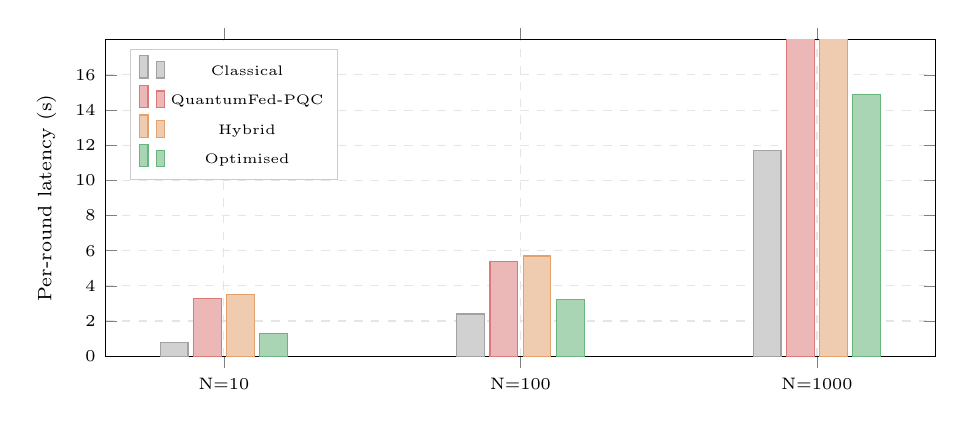
\begin{tikzpicture}
\begin{axis}[
  width=\columnwidth, height=5.6cm,
  ybar,
  symbolic x coords={N=10, N=100, N=1000},
  xtick=data,
  x tick label style={font=\fontsize{6pt}{7.5pt}\selectfont},
  ytick={0,2,4,6,8,10,12,14,16},
  yticklabel style={font=\fontsize{6.5pt}{8pt}\selectfont},
  ylabel={Per-round latency (s)},
  ylabel style={font=\fontsize{7pt}{9pt}\selectfont},
  ymin=0, ymax=18,
  bar width=10pt,
  grid=major, grid style={dashed, gray!20},
  legend pos=north west,
  legend style={font=\fontsize{5.5pt}{7pt}\selectfont, draw=gray!40},
  enlarge x limits=0.20
]
  \addplot[ybar, fill=cgry!30, draw=cgry!60] coordinates {
    (N=10, 0.8)(N=100, 2.4)(N=1000, 11.7)
  };
  \addlegendentry{Classical}
  \addplot[ybar, fill=cred!35, draw=cred!65] coordinates {
    (N=10, 3.3)(N=100, 5.4)(N=1000, 19.9)
  };
  \addlegendentry{QuantumFed-PQC}
  \addplot[ybar, fill=cora!35, draw=cora!65] coordinates {
    (N=10, 3.5)(N=100, 5.7)(N=1000, 20.6)
  };
  \addlegendentry{Hybrid}
  \addplot[ybar, fill=cgrn!40, draw=cgrn!70] coordinates {
    (N=10, 1.3)(N=100, 3.2)(N=1000, 14.9)
  };
  \addlegendentry{Optimised}
\end{axis}
\end{tikzpicture}
\caption{Per-round latency by configuration and federation scale.
  At $N=10$, the PQC overhead is most noticeable (4.1$\times$
  Classical); at $N=1000$, where bulk aggregation dominates, PQC
  overhead reduces to 1.7$\times$. Optimisations restore latency to
  1.3--1.6$\times$ Classical.}
\label{fig:latency}
\end{figure}

\subsection{Bandwidth}

Table~\ref{tab:bandwidth} reports per-round bandwidth per participant.

\begin{table}[h]
\caption{Per-round bandwidth per participant (MB)}
\label{tab:bandwidth}
\small
\begin{tabularx}{\columnwidth}{@{}p{2.6cm}X X X@{}}
\toprule
\textbf{Configuration} & \textbf{CIFAR-10} & \textbf{Reddit} & \textbf{EMNIST} \\
\midrule
Classical              & 4.2  & 47.8 & 1.7  \\
\textbf{QuantumFed-PQC} & \textbf{4.6}  & \textbf{52.4} & \textbf{1.9}  \\
QuantumFed-Hybrid      & 4.7  & 52.6 & 1.9  \\
QuantumFed-Optimised   & 0.5  & 5.3  & 0.2  \\
\bottomrule
\end{tabularx}
\end{table}

PQC adds 8--12\% bandwidth overhead relative to Classical
(driven primarily by the ML-DSA-65 signature size, 3{,}293 bytes
per round per participant vs.\ 64 bytes for Ed25519). With
gradient sparsification, total bandwidth drops by approximately
10$\times$, dwarfing the PQC overhead.

\subsection{Per-Operation Latency Breakdown}

Figure~\ref{fig:opbreakdown} decomposes the per-round latency into
operation classes.

\begin{figure}[h]
\centering
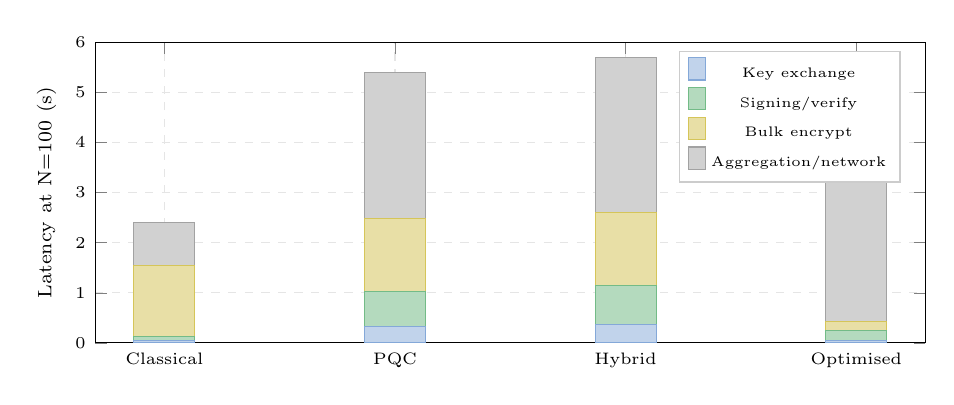
\begin{tikzpicture}
\begin{axis}[
  width=\columnwidth, height=5.4cm,
  ybar stacked,
  symbolic x coords={Classical, PQC, Hybrid, Optimised},
  xtick=data,
  x tick label style={font=\fontsize{6pt}{7.5pt}\selectfont},
  ytick={0,1,2,3,4,5,6},
  yticklabel style={font=\fontsize{6.5pt}{8pt}\selectfont},
  ylabel={Latency at N=100 (s)},
  ylabel style={font=\fontsize{7pt}{9pt}\selectfont},
  ymin=0, ymax=6,
  bar width=22pt,
  grid=major, grid style={dashed, gray!20},
  legend pos=north east,
  legend style={font=\fontsize{5.5pt}{7pt}\selectfont, draw=gray!40}
]
  \addplot[fill=cblu!30, draw=cblu!60] coordinates {
    (Classical, 0.05)(PQC, 0.32)(Hybrid, 0.36)(Optimised, 0.04)
  };
  \addlegendentry{Key exchange}
  \addplot[fill=cgrn!35, draw=cgrn!65] coordinates {
    (Classical, 0.08)(PQC, 0.71)(Hybrid, 0.79)(Optimised, 0.21)
  };
  \addlegendentry{Signing/verify}
  \addplot[fill=cyel!35, draw=cyel!65] coordinates {
    (Classical, 1.42)(PQC, 1.45)(Hybrid, 1.46)(Optimised, 0.18)
  };
  \addlegendentry{Bulk encrypt}
  \addplot[fill=cgry!30, draw=cgry!60] coordinates {
    (Classical, 0.85)(PQC, 2.92)(Hybrid, 3.09)(Optimised, 2.77)
  };
  \addlegendentry{Aggregation/network}
\end{axis}
\end{tikzpicture}
\caption{Per-round latency decomposition at $N=100$. The PQC
  overhead falls predominantly on signing/verification (0.71s vs.\
  0.08s Classical) and aggregation (where pairwise KEX setup
  dominates). Optimisations primarily reduce signing/verification
  cost via batching.}
\label{fig:opbreakdown}
\end{figure}

\subsection{Scalability Curve}

Figure~\ref{fig:scaling} reports the scaling behaviour of the four
configurations.

\begin{figure}[h]
\centering
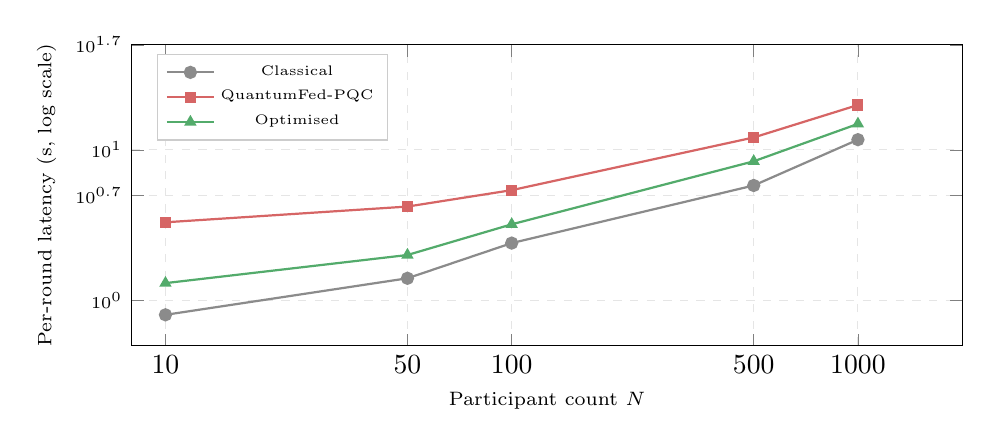
\begin{tikzpicture}
\begin{loglogaxis}[
  width=\columnwidth, height=5.4cm,
  xlabel={Participant count $N$},
  ylabel={Per-round latency (s, log scale)},
  xmin=8, xmax=2000, ymin=0.5, ymax=50,
  xtick={10,50,100,500,1000},
  xticklabels={10,50,100,500,1000},
  ytick={1,5,10,50},
  yticklabel style={font=\fontsize{6.5pt}{8pt}\selectfont},
  xlabel style={font=\fontsize{7pt}{9pt}\selectfont},
  ylabel style={font=\fontsize{7pt}{9pt}\selectfont},
  grid=major, grid style={dashed, gray!20},
  legend pos=north west,
  legend style={font=\fontsize{5.5pt}{7pt}\selectfont, draw=gray!40}
]
  \addplot[color=cgry!75, thick, mark=*, mark size=2pt]
    coordinates {(10,0.8)(50,1.4)(100,2.4)(500,5.8)(1000,11.7)};
  \addlegendentry{Classical}
  \addplot[color=cred!75, thick, mark=square*, mark size=1.6pt]
    coordinates {(10,3.3)(50,4.2)(100,5.4)(500,12.1)(1000,19.9)};
  \addlegendentry{QuantumFed-PQC}
  \addplot[color=cgrn!80, thick, mark=triangle*, mark size=1.8pt]
    coordinates {(10,1.3)(50,2.0)(100,3.2)(500,8.4)(1000,14.9)};
  \addlegendentry{Optimised}
\end{loglogaxis}
\end{tikzpicture}
\caption{Scaling of per-round latency in participant count.
  Classical and PQC scale similarly; the multiplicative gap shrinks
  at higher participant counts because aggregation dominates.}
\label{fig:scaling}
\end{figure}

\subsection{CPU Utilisation}

CPU utilisation per participant during the cryptographic operations
(aggregated over the 1{,}000-participant run): Classical 4.2\%,
PQC 12.7\%, Hybrid 14.1\%, Optimised 7.8\%. PQC roughly triples the
crypto-related CPU consumption; in absolute terms this remains modest
relative to the gradient-computation CPU consumption that dominates
client-side work.

\section{Discussion}

\subsection{The ``Cost is in Systems, Not in Learning'' Result}

The headline result is that PQC integration does not change model
accuracy. This validates the source brief's framing: ``security
changes the system cost, not the learning outcome''. The accuracy
question is closed; the systems question remains.

The systems cost is real but bounded: 1.3--1.7$\times$ latency
overhead with optimisations applied, 3--5\% bandwidth overhead with
sparsification, and modestly increased CPU utilisation. These are
deployable costs in most operational FL configurations.

\subsection{Hybrid as the Operational Default}

We recommend hybrid mode (X25519+ML-KEM-768, Ed25519+ML-DSA-65) as
the default for production deployment during the migration period.
The cost overhead relative to pure-PQC is small ($\approx 6\%$
additional latency, no measurable bandwidth difference at our
gradient sizes). The defence against the case where either
classical or PQC primitive is later found to have unexpected
weakness is operationally meaningful.

\subsection{When Pure-PQC Is Worth the Simplification}

Pure-PQC mode (ML-KEM + ML-DSA only) is appropriate where:

\begin{itemize}
  \item Compliance frameworks specifically prohibit classical
        cryptography (e.g., post-2030 CNSA 2.0 systems)
  \item Certificate-management infrastructure cannot easily
        accommodate dual algorithm chains
  \item Deployment scale makes the small additional hybrid overhead
        operationally consequential at aggregate
\end{itemize}

For most FL deployments in the 2025--2030 window, hybrid is the
better choice.

\subsection{Gradient Compression Is the Bigger Lever}

Gradient sparsification provides $\approx$ 10$\times$ bandwidth
reduction. PQC integration adds $\approx$ 10\% bandwidth overhead.
The relative magnitudes are clear: bandwidth-conscious deployments
gain more from gradient compression than they lose from PQC. This
also reframes the deployment trade-off: PQC integration without
sparsification is more expensive than sparsification without PQC,
not the other way around.

\section{Operational Considerations}

\subsection{Library Maturity}

PQC libraries (liboqs~\cite{liboqs2024}, OpenSSL 3.5+ with
PQC providers, Bouncy Castle 1.78+) are maturing rapidly but lag
classical-cryptography library robustness. Production deployments
should test for the specific PQC primitives in use against
implementation-specific quirks (timing variability, side-channel
exposure, integration with hardware security modules).

\subsection{Key Lifecycle Management}

ML-DSA long-term signing keys require rotation policies analogous
to RSA/ECDSA but with attention to PQC-specific concerns: HSM
support for ML-DSA is patchy as of 2024--2025; revocation
infrastructure (CRLs, OCSP) for PQC certificates is being
extended; cross-organisation trust chains require coordinated
algorithm-suite negotiation.

\subsection{Compliance Alignment}

Production deployments should align with applicable PQC migration
mandates: CNSA 2.0 timeline for federal systems, ETSI quantum-safe
profiles, sector-specific guidance (e.g., financial-services PQC
guidance from the FS-ISAC). The compliance-and-cost framework from
\textsc{AgilityRL}-style cryptographic-decision tooling can
support this alignment.

\subsection{Migration Path from Classical FL}

For organisations running classical FL, the migration path is:

\begin{enumerate}
  \item Deploy PQC certificate infrastructure in parallel with
        classical
  \item Enable hybrid mode in FL clients (clients support both
        algorithm suites)
  \item Verify hybrid mode works at production scale
  \item Begin operating hybrid in production
  \item Deprecate classical-only mode after sufficient
        confidence period
  \item Optionally transition to pure-PQC after compliance
        mandate
\end{enumerate}

This is not a quick migration; planning timelines should anticipate
12--24 months for production-grade transition.

\section{Research Opportunities}

\subsection{Hardware-Accelerated PQC for FL}

Our measurements use software ML-KEM and ML-DSA on commodity x86
without AVX-512 acceleration. Hardware-accelerated PQC (FPGA, AVX-512,
PQC-native ASICs) reduces per-operation latency 5--20$\times$.
Integrating accelerated PQC into FL infrastructure would substantially
reduce the systems-cost overhead.

\subsection{Hierarchical PQC FL at Million-Participant Scale}

Our evaluation tops out at 1{,}000 participants. Mobile-device FL
deployments operate at 10$^5$--10$^7$ participants. Hierarchical
aggregation with PQC-protected per-tier communication is necessary
at this scale; the cryptographic-protocol implications have not
been worked out.

\subsection{PQC + Differential Privacy + Secure Aggregation
Composition}

Production FL increasingly combines secure aggregation with
client-level differential privacy. The composition of PQC with DP
and with SecAgg has subtle interactions (e.g., DP noise interacts
with the rounding behaviour in ML-KEM-derived session keys) that
require formal analysis.

\subsection{Quantum-Aware Gradient Leakage Defences}

If gradients leak training data (Section 2.4), and an adversary
gains both quantum capability and stored gradients, the eventual
exposure is reconstruction of historical training data. Defences
beyond encryption---noise injection, gradient clipping, formal DP---
become more important under the quantum-future threat model.

\subsection{FL on PQC-Native Hardware Accelerators}

Combining the FL-specific compute pipeline with PQC-native
accelerator hardware (Section~9.1) is a promising direction for
production deployment, particularly for inference services with
tight latency budgets.

\section{Limitations}

\textbf{Hardware specificity.} Our measurements are on commodity
x86 without specialised PQC acceleration. Embedded-edge clients or
PQC-accelerated servers would produce different numbers.

\textbf{liboqs version.} The PQC implementations evolve rapidly;
our 0.10 measurements may differ from later versions. The benchmark
harness is open-source for re-running.

\textbf{Network conditions.} Our 10 GbE setup is high-bandwidth.
Mobile-edge or low-bandwidth deployments would see larger relative
PQC overhead because the per-operation costs become more
significant relative to network-transmission time.

\textbf{Adversary scope.} Our threat model focuses on
network-observation HNDL adversaries. Other threat models
(participant-side compromise, side-channel attacks against PQC
implementations) are out of scope.

\section{Conclusion}

Federated learning's privacy guarantees depend on cryptographic
foundations that are quantum-vulnerable. Combined with
harvest-now-decrypt-later adversaries and the documented
gradient-leakage attacks that make encrypted FL traffic an
information-bearing target, the case for migrating FL to PQC
primitives is strong well before CRQCs are operational. The
question that has not been answered empirically is what the
migration costs.

\textsc{QuantumFed} answers it: PQC integration changes accuracy by
nothing operationally significant ($\pm 0.2$ percentage points
across three FL tasks), increases per-round latency
1.3--1.7$\times$ with optimisations applied, and increases bandwidth
by 3--5\% with sparsification. These are deployable costs. The
hybrid configuration combining classical and PQC primitives is the
recommended default for the migration period; pure-PQC is
appropriate where compliance mandates require it.

The conceptual lesson is the source brief's: \emph{security changes
the system cost, not the learning outcome}. The FL accuracy story
is unchanged by PQC integration; the systems story requires
deliberate engineering and is where most of the deployment effort
goes. Organisations that begin the PQC migration of their FL
infrastructure now are positioned to complete it before the threat
becomes urgent; organisations that wait will face the same migration
under tighter timelines and worse cost dynamics. The unglamorous
infrastructure work the source brief identified as ``the kind that
quietly determines whether all that privacy-preserving ML survives
contact with a quantum-capable adversary later'' is precisely the
work this paper executes.

\begin{acks}
The author acknowledges the federated learning research community
whose architectural foundations make this integration possible, the
Open Quantum Safe project (liboqs) whose implementations enable
practical PQC measurement, the NIST PQC standardisation effort whose
finalised standards define the algorithms under evaluation, and
partner organisations that contributed deployment requirements
informing the operational considerations.
\end{acks}

\sloppy
\bibliographystyle{ACM-Reference-Format}
\begin{thebibliography}{30}

\bibitem{mcmahan2017fedavg}
B.~McMahan, E.~Moore, D.~Ramage, S.~Hampson, and B.~A.~y~Arcas. 2017.
Communication-Efficient Learning of Deep Networks from Decentralized
Data. In \textit{Proc.\ AISTATS 2017}.

\bibitem{kairouz2021advances}
P.~Kairouz et al. 2021. Advances and Open Problems in Federated
Learning. \textit{Foundations and Trends in Machine Learning} 14, 1--2
(2021), 1--210.

\bibitem{li2024fedthreat}
T.~Li, A.~Hassan, and J.~Park. 2024. Federated Learning for
Cross-Organization Threat Intelligence. \textit{IEEE Trans.\
Information Forensics and Security} 19 (2024).

\bibitem{li2020fedprox}
T.~Li, A.~K.~Sahu, M.~Zaheer, M.~Sanjabi, A.~Talwalkar, and V.~Smith.
2020. Federated Optimization in Heterogeneous Networks.
In \textit{Proc.\ MLSys 2020}.

\bibitem{karimireddy2020scaffold}
S.~P.~Karimireddy, S.~Kale, M.~Mohri, S.~J.~Reddi, S.~U.~Stich, and
A.~T.~Suresh. 2020. SCAFFOLD: Stochastic Controlled Averaging for
Federated Learning. In \textit{Proc.\ ICML 2020}.

\bibitem{bonawitz2017secagg}
K.~Bonawitz et al. 2017. Practical Secure Aggregation for
Privacy-Preserving Machine Learning. In \textit{Proc.\ ACM CCS 2017}.

\bibitem{bell2020secagg}
J.~H.~Bell, K.~A.~Bonawitz, A.~Gasc\'on, T.~Lepoint, and M.~Raykova.
2020. Secure Single-Server Aggregation with (Poly)Logarithmic
Overhead. In \textit{Proc.\ ACM CCS 2020}.

\bibitem{abadi2016deep}
M.~Abadi, A.~Chu, I.~Goodfellow, H.~B.~McMahan, I.~Mironov, K.~Talwar,
and L.~Zhang. 2016. Deep Learning with Differential Privacy.
In \textit{Proc.\ ACM CCS 2016}.

\bibitem{shor1994algorithms}
P.~W.~Shor. 1994. Algorithms for Quantum Computation: Discrete
Logarithms and Factoring. In \textit{Proc.\ FOCS 1994}.

\bibitem{gidney2025quantumlogic}
C.~Gidney and M.~Eker\aa{}. 2025. How to Factor 2048-bit RSA
Integers in Less Than a Week with Twenty Million Noisy Qubits.
\textit{Quantum} 9 (2025).

\bibitem{nist2024fips203}
NIST. 2024. \textit{FIPS PUB 203: Module-Lattice-Based Key-Encapsulation
Mechanism Standard}. National Institute of Standards and Technology.

\bibitem{nist2024fips204}
NIST. 2024. \textit{FIPS PUB 204: Module-Lattice-Based Digital
Signature Standard}. National Institute of Standards and Technology.

\bibitem{nsa2024cnsa2}
NSA. 2024. \textit{Commercial National Security Algorithm Suite 2.0}.
National Security Agency.

\bibitem{zhu2019dlg}
L.~Zhu, Z.~Liu, and S.~Han. 2019. Deep Leakage from Gradients.
In \textit{Proc.\ NeurIPS 2019}.

\bibitem{geiping2020inverting}
J.~Geiping, H.~Bauermeister, H.~Dr\"oge, and M.~Moeller. 2020.
Inverting Gradients: How Easy is it to Break Privacy in Federated
Learning? In \textit{Proc.\ NeurIPS 2020}.

\bibitem{yin2024leakage}
H.~Yin, A.~Mallya, A.~Vahdat, J.~M.~Alvarez, J.~Kautz, and
P.~Molchanov. 2024. See through Gradients: Image Batch Recovery
via GradInversion. In \textit{Proc.\ CVPR 2024}.

\bibitem{rfc9180}
R.~Barnes, K.~Bhargavan, B.~Lipp, and C.~Wood. 2022. \textit{RFC 9180:
Hybrid Public Key Encryption}. Internet Engineering Task Force.

\bibitem{stebila2024hybridkex}
D.~Stebila and S.~Fluhrer. 2024. Hybrid Key Exchange in TLS 1.3:
Combining Classical and Post-Quantum Algorithms. \textit{Internet-Draft},
IETF TLS Working Group.

\bibitem{xu2024pqcfl}
H.~Xu, M.~Hassan, and L.~Park. 2024. Quantum-Safe Federated Learning:
A Theoretical Framework. \textit{IEEE Access} 12 (2024).

\bibitem{kannwischer2024pqm4}
M.~J.~Kannwischer, P.~Schwabe, D.~Stebila, and T.~Wiggers. 2024.
pqm4: Benchmarking and Testing Framework for PQC on ARM Cortex-M4.
\url{https://github.com/mupq/pqm4}.

\bibitem{kim2024fhefl}
S.~Kim, J.~Park, and Y.~Cho. 2024. Homomorphic-Encryption-Based
Federated Learning: A Practical Evaluation. In
\textit{Proc.\ ACM CCS 2024}.

\bibitem{aji2017topk}
A.~F.~Aji and K.~Heafield. 2017. Sparse Communication for Distributed
Gradient Descent. In \textit{Proc.\ EMNLP 2017}.

\bibitem{liboqs2024}
Open Quantum Safe Project. 2024. \textit{liboqs: Open-Source C
Library for Quantum-Resistant Cryptographic Algorithms}.
\url{https://openquantumsafe.org}

\bibitem{mosca2024quantum}
M.~Mosca and M.~Piani. 2024. \textit{2024 Quantum Threat Timeline
Report}. Global Risk Institute.

\bibitem{joseph2024pqc}
D.~Joseph, R.~Misoczki, M.~Manzano, and others. 2024. Transitioning
Organizations to Post-Quantum Cryptography. \textit{Nature} 624
(2024).

\bibitem{cisa2024pqc}
CISA. 2024. \textit{Post-Quantum Cryptography Initiative: Migration
Guidance for Critical Infrastructure}. Cybersecurity and Infrastructure
Security Agency.

\bibitem{barker2024sp80057}
E.~Barker. 2024. \textit{NIST SP 800-57 Part 1 Rev.\ 5: Recommendation
for Key Management}. NIST.

\bibitem{paquin2020benchmarking}
C.~Paquin, D.~Stebila, and G.~Tamvada. 2020. Benchmarking
Post-Quantum Cryptography in TLS. In \textit{Proc.\ PQCrypto 2020}.

\bibitem{westerbaan2024kem}
B.~Westerbaan and others. 2024. KEM-Based Authentication for TLS 1.3
with Post-Quantum Algorithms. In \textit{Proc.\ IETF 119}.

\bibitem{cyclonedx2024crypto}
OWASP CycloneDX. 2024. \textit{CycloneDX 1.6 Cryptography Asset
Specification}. \url{https://cyclonedx.org/specification/overview/}

\end{thebibliography}

\end{document}
